\chapter{O projeto do produto} 
\label{chap:projeto_do_produto} 

Existem diversos tipos de projetos necessários à implementação e funcionamento de uma empresa industrial. No presente capítulo, será focado em demonstrar como o projeto do produto pode ser fornecido pela empresa. Essa atividade parte da etapa inicial (Conceito, triagem do conceito, projeto preliminar, avaliação do projeto preliminar, construção de protótipos e projeto final do produto), passa pela documentação final resultante do projeto do produto até chegar na gestão do projeto de novos produtos. No final desta seção será mostrado como a \textit{SunBurn} utilizou destes conceitos para conceber o seu produto.

\section{Sec1} 
\label{sec:projeto_do_produto_sec1} 

Para conceber um projeto final de um produto é necessário que o projeto passe por diversas etapas fundamentais. Com isso, um fluxograma é formado como mostrado na Figura \ref{fig:projeto_produto}, mesmo que, na prática os projetistas avancem ou retrocedam pelas etapas. Serão descritas a seguir cada etapa deste processo na ordem em que geralmente ocorrem.

\begin{figure}[H]
  \centering
  \caption{Fluxograma das etapas do projeto do produto.}
  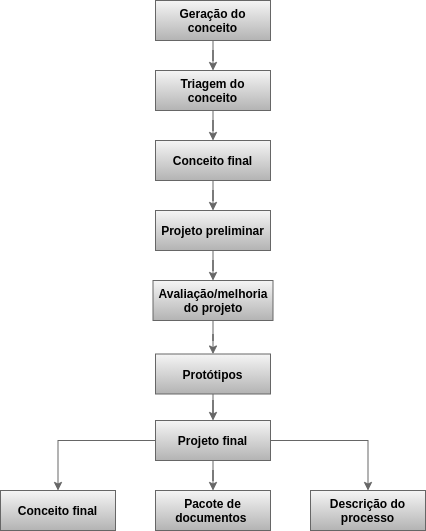
\includegraphics[width=1\textwidth]{images/projeto_produto.png}
  \caption*{Fonte: Adaptado \cite{slack2006administracao} }
  \label{fig:projeto_produto}
\end{figure}



\section{Aplicação Prática} 
\label{sec:projeto_do_produto_aplicacao}